
%{{第三十八回}}{第三十八回}}

\chapter{林潇湘魁夺菊花诗\hspace{.5em}薛蘅芜讽和螃蟹咏}

{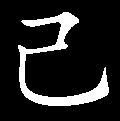
\includegraphics[width=3mm]{../Images/00003}  \kaishu 题曰``菊花诗''、``螃蟹咏'',偏自太君前阿凤若许诙谐中不失体、鸳鸯平儿宠婢中多少放肆之迎合取乐写来,似难入题,却轻轻用弄水戏鱼看花等游玩事及王夫人云``这里风大''一句收住入题,并无纤毫牵强。此重作轻抹法也。妙极,好看煞!}

话说宝钗湘云二人计议已妥,一宿无话。湘云次日便请贾母等赏桂花。贾母等都说道:``是他有兴头,须要扰他这雅兴。''{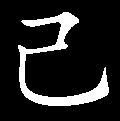
\includegraphics[width=3mm]{../Images/00003}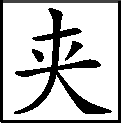
\includegraphics[width=3mm]{../Images/00012}\footnotesize \kaishu 若在世俗小家,则云:``你是客,在我们舍下,怎么反扰你的?''一何可笑。}至午,果然贾母带了王夫人凤姐兼请薛姨妈等进园来。贾母因问:``那一处好?''{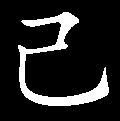
\includegraphics[width=3mm]{../Images/00003}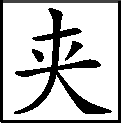
\includegraphics[width=3mm]{../Images/00012}\footnotesize \kaishu 必如此问方好。}王夫人道:``凭老太太爱在那一处,就在那一处。''{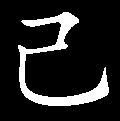
\includegraphics[width=3mm]{../Images/00003}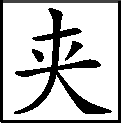
\includegraphics[width=3mm]{../Images/00012}\footnotesize \kaishu 必是王夫人如此答方妙。}凤姐道:``藕香榭已经摆下了,那山坡下两颗桂花开的又好,河里的水又碧清,坐在河当中亭子上岂不敞亮,看着水眼也清亮。''{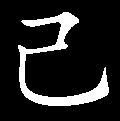
\includegraphics[width=3mm]{../Images/00003}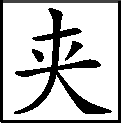
\includegraphics[width=3mm]{../Images/00012}\footnotesize \kaishu 智者乐水,岂其然乎?}贾母听了,说:``这话很是。''说着,就引了众人往藕香榭来。原来这藕香榭盖在池中,四面有窗,左右有曲廊可通,亦是跨水接岸,后面又有曲折竹桥暗接。众人上了竹桥,凤姐忙上来搀着贾母,口里说:``老祖宗只管迈大步走,不相干的,这竹子桥规矩是咯吱咯喳的。''{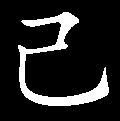
\includegraphics[width=3mm]{../Images/00003}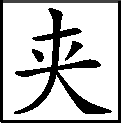
\includegraphics[width=3mm]{../Images/00012}\footnotesize \kaishu 如见其势,如临其上,非走过者必形容不出。}

一时进入榭中,只见栏杆外另放着两张竹案,一个上面设着杯箸酒具,一个上头设着茶筅茶盂各色茶具。那边有两三个丫头煽风炉煮茶,这一边另外几个丫头也煽风炉烫酒呢。贾母喜的忙问:``这茶想的到,且是地方,东西都干净。''湘云笑道:``这是宝姐姐帮着我预备的。''贾母道:``我说这个孩子细致,凡事想的妥当。''一面说,一面又看见柱上挂的黑漆嵌蚌的对子,命人念。湘云念道:

芙蓉影破归兰桨,菱藕香深写竹桥。{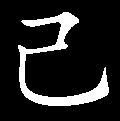
\includegraphics[width=3mm]{../Images/00003}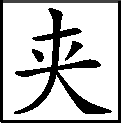
\includegraphics[width=3mm]{../Images/00012}\footnotesize \kaishu 妙极!此处忽又补出一处,不入贾政``试才''一回,皆错综其事,不作一直笔也。}

贾母听了,又抬头看匾,因回头向薛姨妈道:``我先小时,家里也有这么一个亭子,叫做什么`枕霞阁'。我那时也只像他们这么大年纪,同姊妹们天天顽去。那日谁知我失了脚掉下去,几乎没淹死,好容易救了上来,到底被那木钉把头碰破了。如今这鬓角上那指头顶大一块窝儿就是那残破了。众人都怕经了水,又怕冒了风,都说活不得了,谁知竟好了。''

凤姐不等人说,先笑道:``那时要活不得,如今这大福可叫谁享呢!可知老祖宗从小儿的福寿就不小,神差鬼使碰出那个窝儿来,好盛福寿的。寿星老儿头上原是一个窝儿,因为万福万寿盛满了,所以倒凸高出些来了。''未及说完,贾母与众人都笑软了。{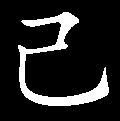
\includegraphics[width=3mm]{../Images/00003}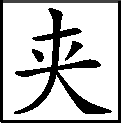
\includegraphics[width=3mm]{../Images/00012}\footnotesize \kaishu 看他忽用贾母数语,闲闲又补出此书之前似已有一部《十二钗》的一般,令人遥忆不能一见,余则将欲补出枕霞阁中十二钗来,岂不又添一部新书?}贾母笑道:``这猴儿惯的了不得了,只管拿我取笑起来,恨的我撕你那油嘴。''凤姐笑道:``回来吃螃蟹,恐积了冷在心里,讨老祖宗笑一笑开开心,一高兴多吃两个就无妨了。''贾母笑道:``明儿叫你日夜跟着我,我倒常笑笑觉的开心,不许回家去。''王夫人笑道:``老太太因为喜欢他,才惯的他这样,还这样说,他明儿越发无礼了。''贾母笑道:``我喜欢他这样,况且他又不是那不知高低的孩子。家常没人,娘儿们原该这样。横竖礼体不错就罢,没的倒叫他从神儿似的作什么。''{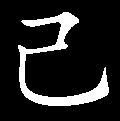
\includegraphics[width=3mm]{../Images/00003}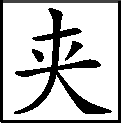
\includegraphics[width=3mm]{../Images/00012}\footnotesize \kaishu 近之暴发专讲{(理)}{[}礼{]}法,竟不知礼法,此似无礼而礼法井井,所谓``整瓶不动半瓶摇'',又曰``习惯成自然'',真不谬也。}

说着,一齐进入亭子,献过茶,凤姐忙着搭桌子,要杯箸。上面一桌,贾母、薛姨妈、宝钗、黛玉、宝玉;东边一桌,史湘云、王夫人、迎、探、惜;西边靠门一桌,李纨和凤姐的,虚设坐位,二人皆不敢坐,只在贾母王夫人两桌上伺候。凤姐吩咐:``螃蟹不可多拿来,仍旧放在蒸笼里,拿十个来,吃了再拿。''一面又要水洗了手,站在贾母跟前剥蟹肉,头次让薛姨妈。薛姨妈道:``我自己掰着吃香甜,不用人让。''凤姐便奉与贾母。二次的便与宝玉,又说:``把酒烫的滚热的拿来。''又命小丫头们去取了菊花叶儿、桂花蕊熏的绿豆面子来,预备着洗手。史湘云陪着吃了一个,就下座来让人,又出至外头,令人盛两盘子与赵姨娘周姨娘送去。又见凤姐走来道:``你不惯张罗,你吃你的去。我先替你张罗,等散了我再吃。''湘云不肯,又令人在那边廊上摆了两桌,让鸳鸯、琥珀、彩霞、彩云、平儿去坐。鸳鸯因向凤姐笑道:``二奶奶在这里伺候,我们可吃去了。''凤姐儿道:``你们只管去,都交给我就是了。''说着,史湘云仍入了席。凤姐和李纨也胡乱应个景儿。

凤姐仍是下来张罗,一时出至廊上,鸳鸯等正吃的高兴,见他来了,鸳鸯等站起来道:``奶奶又出来作什么?让我们也受用一会子。''凤姐笑道:``鸳鸯小蹄子越发坏了,我替你当差,倒不领情,还抱怨我。还不快斟一钟酒来我喝呢。''鸳鸯笑着忙斟了一杯酒,送至凤姐唇边,凤姐一扬脖子吃了。琥珀、彩霞二人也斟上一杯,送到凤姐唇边,那凤姐也吃了。\href{../Text/part0042_split_000.html\#lnkback_1_a}{\textsuperscript{①}}平儿早剔了一壳黄子送来,凤姐道:``多倒些姜醋。''一面也吃了,笑道:``你们坐着吃罢,我可去了。''

鸳鸯笑道:``好没脸,吃我们的东西。''凤姐儿笑道:``你和我少作怪。你知道你琏二爷爱上了你,要和老太太讨了你做小老婆呢。''鸳鸯道:``啐,这也是作奶奶说出来的话!我不拿腥手抹你一脸算不得。''说着赶来就要抹。凤姐儿央道:``好姐姐,饶我这一遭儿罢。''琥珀笑道:``鸳丫头要去了,平丫头还饶他?你们看看他,没有吃了两个螃蟹,倒喝了一碟子醋,他也算不会揽酸了。''平儿手里正掰了个满黄的螃蟹,听如此奚落他,便拿着螃蟹照着琥珀脸上抹来,口内笑骂``我把你这嚼舌根的小蹄子!''琥珀也笑着往旁边一躲,平儿使空了,往前一撞,正恰恰的抹在凤姐儿腮上。凤姐儿正和鸳鸯嘲笑,不防唬了一跳,``嗳哟''了一声。众人撑不住都哈哈的大笑起来。凤姐也禁不住笑骂道:``死娼妇!吃离了眼了,混抹你娘的。''平儿忙赶过来替他擦了,亲自去端水。鸳鸯道:``阿弥陀佛!这是个报应。''

贾母那边听见,一叠声问:``见了什么这样乐,告诉我们也笑笑。''鸳鸯等忙高声笑回道:``二奶奶来抢螃蟹吃,平儿恼了,抹了他主子一脸的螃蟹黄子。主子奴才打架呢。''贾母和王夫人等听了也笑起来。贾母笑道:``你们看他可怜见的,把那小腿子脐子给他点子吃也就完了。''鸳鸯等笑着答应了,高声又说道:``这满桌子的腿子,二奶奶只管吃就是了。''凤姐洗了脸走来,又伏侍贾母等吃了一回。黛玉独不敢多吃,只吃了一点儿夹子肉就下来了。

贾母一时不吃了,大家方散,都洗了手,也有看花的,也有弄水看鱼的,游玩了一回。王夫人因回贾母说:``这里风大,才又吃了螃蟹,老太太还是回房去歇歇罢了。若高兴,明日再来逛逛。''贾母听了,笑道:``正是呢。我怕你们高兴,我走了又怕扫了你们的兴。既这么说,咱们就都去吧。''回头又嘱咐湘云:``别让你宝哥哥、林姐姐多吃了。''湘云答应着。又嘱咐湘云、宝钗二人说:``你两个也别多吃。那东西虽好吃,不是什么好的,吃多了肚子疼。''二人忙应着送出园外,仍旧回来,令将残席收拾了另摆。宝玉道:``也不用摆,咱们且作诗。把那大团圆桌就放在当中,酒菜都放着。也不必拘定坐位,有爱吃的大家去吃,散坐岂不便宜。''宝钗道:``这话极是。''湘云道:``虽如此说,还有别人。''因又命另摆一桌,拣了热螃蟹来,请袭人、紫鹃、司棋、待书、入画、莺儿、翠墨等一处共坐。山坡桂树底下铺下两条花毡,命答应的婆子并小丫头等也都坐了,只管随意吃喝,等使唤再来。

湘云便取了诗题,用针绾在墙上。众人看了,都说:``新奇固新奇,只怕作不出来。''湘云又把不限韵的原故说了一番。宝玉道:``这才是正理,我也最不喜限韵。''林黛玉因不大吃酒,又不吃螃蟹,自令人掇了一个绣墩倚栏杆坐着,拿着钓竿钓鱼。宝钗手里拿着一枝桂花玩了一回,俯在窗槛上掐了桂蕊掷向水面,引的游鱼浮上来唼喋。湘云出一回神,又让一回袭人等,又招呼山坡下的众人只管放量吃。探春和李纨惜春立在垂柳阴中看鸥鹭。迎春又独在花阴下拿着花针穿茉莉花。{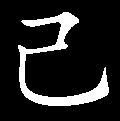
\includegraphics[width=3mm]{../Images/00003}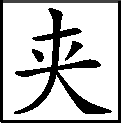
\includegraphics[width=3mm]{../Images/00012}\footnotesize \kaishu 看他各人各式,亦如画家有孤耸独出,则有攒三聚五,疏疏密密,直是一幅《百美图》。}宝玉又看了一回黛玉钓鱼,一回又俯在宝钗旁边说笑两句,一回又看袭人等吃螃蟹,自己也陪他饮两口酒。袭人又剥一壳肉给他吃。

黛玉放下钓竿,走至座间,拿起那乌银梅花自斟壶来,{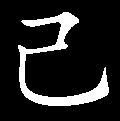
\includegraphics[width=3mm]{../Images/00003}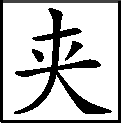
\includegraphics[width=3mm]{../Images/00012}\footnotesize \kaishu 写壶非写壶,正写黛玉。}拣了一个小小的海棠冻石蕉叶杯。{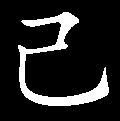
\includegraphics[width=3mm]{../Images/00003}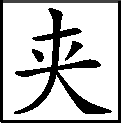
\includegraphics[width=3mm]{../Images/00012}\footnotesize \kaishu 妙杯!非写杯,正写黛玉。``拣''字有神理,盖黛玉不善饮,此任性也。}丫鬟看见,知他要饮酒,忙着走上来斟。黛玉道:``你们只管吃去,让我自斟,这才有趣儿。''说着便斟了半盏,看时却是黄酒,因说道:``我吃了一点子螃蟹,觉得心口微微的疼,须得热热的喝口烧酒。''宝玉忙道:``有烧酒。''便令将那合欢花浸的酒烫一壶来。{{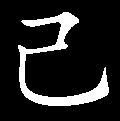
\includegraphics[width=3mm]{../Images/00003}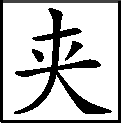
\includegraphics[width=3mm]{../Images/00012}\footnotesize \kaishu 伤哉!作者犹记矮}?{舫前以合欢花酿酒乎?屈指二十年矣。}}黛玉也只吃了一口便放下了。

宝钗也走过来,另拿了一只杯来,也饮了一口,便蘸笔至墙上把头一个《忆菊》勾了,底下又赘了一个``蘅''字。{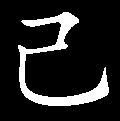
\includegraphics[width=3mm]{../Images/00003}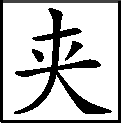
\includegraphics[width=3mm]{../Images/00012}\footnotesize \kaishu 妙极韵极!}宝玉忙道:``好姐姐,第二个我已经有了四句了,你让我作罢。''宝钗笑道:``我好容易有了一首,你就忙的这样。''黛玉也不说话,接过笔来把第八个《问菊》勾了,接着把第十一个《菊梦》也勾了,也赘一个``潇''字。{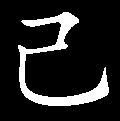
\includegraphics[width=3mm]{../Images/00003}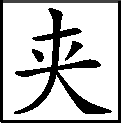
\includegraphics[width=3mm]{../Images/00012}\footnotesize \kaishu 这两个妙题,料定黛卿必喜,岂让他人作去哉?}宝玉也拿起笔来,将第二个《访菊》也勾了,也赘上一个``绛''字。探春走来看看道:``竟没有人作《簪菊》,让我作这《簪菊》。''又指着宝玉笑道:``才宣过总不许带出闺阁字样来,你可要留神。''

说着,只见史湘云走来,将第四第五《对菊》《供菊》一连两个都勾了,也赘上一个``湘''字。探春道:``你也该起个号。''湘云笑道:``我们家里如今虽有几处轩馆,我又不住着,借了来也没趣。''{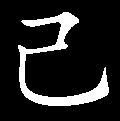
\includegraphics[width=3mm]{../Images/00003}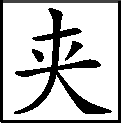
\includegraphics[width=3mm]{../Images/00012}\footnotesize \kaishu 近之不读书暴发户偏爱起一别号。一笑。}宝钗笑道:``方才老太太说,你们家也有这个水亭叫`枕霞阁',难道不是你的。如今虽没了,你到底是旧主人。''众人都道有理,宝玉不待湘云动手,便代将``湘''字抹了,改了一个``霞''字。

又有顿饭工夫,十二题已全,各自誊出来,都交与迎春,另拿了一张雪浪笺过来,一并誊录出来,某人作的底下赘明某人的号。李纨等从头看起:

忆菊 蘅芜君{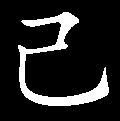
\includegraphics[width=3mm]{../Images/00003}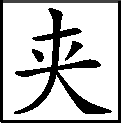
\includegraphics[width=3mm]{../Images/00012}\footnotesize \kaishu 真用此号,妙极!}

怅望西风抱闷思,蓼红苇白断肠时。

空篱旧圃秋无迹,瘦月清霜梦有知。

念念心随归雁远,寥寥坐听晚砧痴。

谁怜我为黄花病,慰语重阳会有期。

访菊 怡红公子

闲趁霜晴试一游,酒杯药盏莫淹留。

霜前月下谁家种,槛外篱边何处秋。

蜡屐远来情得得,冷吟不尽兴悠悠。

黄花若解怜诗客,休负今朝挂杖头。

种菊 怡红公子

携锄秋圃自移来,篱畔庭前故故栽。

昨夜不期经雨活,今朝犹喜带霜开。

冷吟秋色诗千首,醉酹寒香酒一杯。

泉溉泥封勤护惜,好知井迳绝尘埃。

对菊 枕霞旧友

别圃移来贵比金,一丛浅淡一丛深。

萧疏篱畔科头坐,清冷香中抱膝吟。

数去更无君傲世,看来惟有我知音。

秋光荏苒休辜负,相对原宜惜寸阴。

供菊 枕霞旧友

弹琴酌酒喜堪俦,几案婷婷点缀幽。

隔座香分三径露,抛书人对一枝秋。

霜清纸帐来新梦,圃冷斜阳忆旧游。

傲世也因同气味,春风桃李未淹留。

咏菊 潇湘妃子

无赖诗魔昏晓侵,绕篱欹石自沉音。

毫端蕴秀临霜写,口齿噙香对月吟。

满纸自怜题素怨,片言谁解诉秋心。

一从陶令平章后,千古高风说到今。

画菊 蘅芜君

诗馀戏笔不知狂,岂是丹青费较量。

聚叶泼成千点墨,攒花染出几痕霜。

淡浓神会风前影,跳脱秋生腕底香。

莫认东篱闲采掇,粘屏聊以慰重阳。

问菊 潇湘妃子

欲讯秋情众莫知,喃喃负手叩东篱。

孤标傲世偕谁隐,一样花开为底迟?

圃露庭霜何寂寞,雁归蛩病可相思?

休言举世无谈者,解语何妨片语时。

簪菊 蕉下客

瓶供篱栽日日忙,折来休认镜中妆。

长安公子因花癖,彭泽先生是酒狂。

短鬓冷沾三径露,葛巾香染九秋霜。

高情不入时人眼,拍手凭他笑路旁。

菊影 枕霞旧友

秋光叠叠复重重,潜度偷移三径中。

窗隔疏灯描远近,篱筛破月锁玲珑。

寒芳留照魂应驻,霜印传神梦也空。

珍重暗香休踏碎,凭谁醉眼认朦胧。

菊梦 潇湘妃子

篱畔秋酣一觉清,和云伴月不分明。

登仙非慕庄生蝶,忆旧还寻陶令盟。

睡去依依随雁断,惊回故故恼蛩鸣。

醒时幽怨同谁诉,衰草寒烟无限情。

残菊 蕉下客

露凝霜重渐倾欹,宴赏才过小雪时。

蒂有馀香金淡泊,枝无全叶翠离披。

半床落月蛩声病,万里寒云雁阵迟。

明岁秋风知再会,暂时分手莫相思。

众人看一首,赞一首,彼此称扬不已。李纨笑道:``等我从公评来。通篇看来,各有各人的警句。今日公评:《咏菊》第一,《问菊》第二,《菊梦》第三,题目新,诗也新,立意更新,恼不得要推潇湘妃子为魁了;然后《簪菊》《对菊》《供菊》《画菊》《忆菊》次之。''宝玉听说,喜的拍手叫``极是,极公道。''黛玉道:``我那首也不好,到底伤于纤巧些。''李纨道:``巧的却好,不露堆砌生硬。''

黛玉道:``据我看来,头一句好的是`圃冷斜阳忆旧游',这句背面傅粉。`抛书人对一枝秋'已经妙绝,将供菊说完,没处再说,故翻回来想到未折未供之先,意思深透。''李纨笑道:``固如此说,你的`口齿噙香'句也敌的过了。''探春又道:``到底要算蘅芜君沉着,`秋无迹'、`梦有知',把个忆字竟烘染出来了。''宝钗笑道:``你的`短鬓冷沾'、`葛巾香染',也就把簪菊形容的一个缝儿也没了。''湘云道:``\,`偕谁隐'、`为底迟',真个把个菊花问的无言可对。''李纨笑道:``你的`科头坐'、`抱膝吟',竟一时也不能别开,菊花有知,也必腻烦了。''说的大家都笑了。

宝玉笑道:``我又落第。难道`谁家种'、`何处秋'、`蜡屐远来'、`冷吟不尽'都不是访,`昨夜雨'、`今朝霜'都不是种不成?但恨敌不上`口齿噙香对月吟'、`清冷香中抱膝吟'、`短鬓'、`葛巾'、`金淡泊'、`翠离披'、`秋无迹'、`梦有知'这几句罢了。''{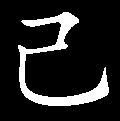
\includegraphics[width=3mm]{../Images/00003}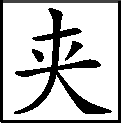
\includegraphics[width=3mm]{../Images/00012}\footnotesize \kaishu 总写宝玉不及,妙极!}又道:``明儿闲了,我一个人作出十二首来。''李纨道:``你的也好,只是不及这几句新巧就是了。''

大家又评了一回,复又要了热蟹来,就在大圆桌子上吃了一回。宝玉笑道:``今日持螯赏桂,亦不可无诗。{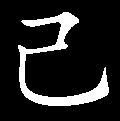
\includegraphics[width=3mm]{../Images/00003}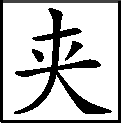
\includegraphics[width=3mm]{../Images/00012}\footnotesize \kaishu 全是他忙,全是他不及。妙极!}我已吟成,谁还敢作呢?''说着,便忙洗了手提笔写出。{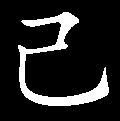
\includegraphics[width=3mm]{../Images/00003}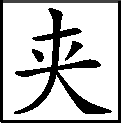
\includegraphics[width=3mm]{../Images/00012}\footnotesize \kaishu 且莫看诗,只看他偏于如许一大回诗后又写一回诗,岂世人想的到的?}众人看道:

持螯更喜桂阴凉,泼醋擂姜兴欲狂。

饕餮王孙应有酒,横行公子却无肠。

脐间积冷馋忘忌,指上沾腥洗尚香。

原为世人美口腹,坡仙曾笑一生忙。

黛玉笑道:``这样的诗,要一百首也有。''{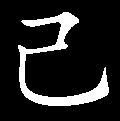
\includegraphics[width=3mm]{../Images/00003}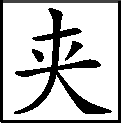
\includegraphics[width=3mm]{../Images/00012}\footnotesize \kaishu 看他这一说。}宝玉笑道:``你这会子才力已尽,不说不能作了,还贬人家。''黛玉听了,并不答言,也不思索,提起笔来一挥,已有了一首。众人看道:

铁甲长戈死未忘,堆盘色相喜先尝。

螯封嫩玉双双满,壳凸红脂块块香。

多肉更怜卿八足,助情谁劝我千觞。{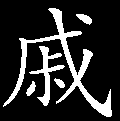
\includegraphics[width=3mm]{../Images/00005}  \kaishu 不脱自己身分。}

对斯佳品酬佳节,桂拂清风菊带霜。

宝玉看了正喝彩,黛玉便一把撕了,令人烧去,因笑道:``我的不及你的,我烧了他。你那个很好,比方才的菊花诗还好,你留着他给人看。''宝钗接着笑道:``我也勉强了一首,未必好,写出来取笑儿罢。''说着也写了出来。大家看时,写道是:

桂霭桐阴坐举觞,长安涎口盼重阳。

眼前道路无经纬,皮里春秋空黑黄。

看到这里,众人不禁叫绝。宝玉道:``写得痛快!我的诗也该烧了。''又看底下道:

酒未敌腥还用菊,性防积冷定须姜。

于今落釜成何益,月浦空馀禾黍香。

众人看毕,都说这是食螃蟹绝唱,这些小题目,原要寓大意才算是大才,只是讽刺世人太毒了些。说着,只见平儿复进园来。不知作什么,且听下回分解。

{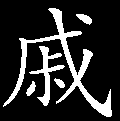
\includegraphics[width=3mm]{../Images/00005}  \kaishu 总评:请看此回中,闺中儿女能作此等豪情韵事,且笔下各能自尽其性情,毫不乖舛。作者之锦心绣口,无庸赘渎。其用意之深,奖劝之勤,读此文者,亦不得轻忽,戒之。}

{\href{../Text/part0042_split_000.html\#navto_1_a}{①}``琥珀\ldots{}\ldots{}那凤姐也吃了。''一句,杨本无。按:鸳鸯等在廊上吃,凤姐在亭里侍候,本不依礼。故鸳鸯也是凤姐索讨才给斟酒的,琥珀、彩霞二人不必响应。否则,这里仅五人,独彩云无表示,也不合适。当以杨本为是。}
